%%%%%%%%%%%%%%%%%%%%%%%%%%%%%%%%%%%%%%%%%%%%%%%%%%%%%%%%%%%%%%%%%%%%%%%%%%%%%%%%
% Template for USENIX papers.
%
% History:
%
% - TEMPLATE for Usenix papers, specifically to meet requirements of
%   USENIX '05. originally a template for producing IEEE-format
%   articles using LaTeX. written by Matthew Ward, CS Department,
%   Worcester Polytechnic Institute. adapted by David Beazley for his
%   excellent SWIG paper in Proceedings, Tcl 96. turned into a
%   smartass generic template by De Clarke, with thanks to both the
%   above pioneers. Use at your own risk. Complaints to /dev/null.
%   Make it two column with no page numbering, default is 10 point.
%
% - Munged by Fred Douglis <douglis@research.att.com> 10/97 to
%   separate the .sty file from the LaTeX source template, so that
%   people can more easily include the .sty file into an existing
%   document. Also changed to more closely follow the style guidelines
%   as represented by the Word sample file.
%
% - Note that since 2010, USENIX does not require endnotes. If you
%   want foot of page notes, don't include the endnotes package in the
%   usepackage command, below.
% - This version uses the latex2e styles, not the very ancient 2.09
%   stuff.
%
% - Updated July 2018: Text block size changed from 6.5" to 7"
%
% - Updated Dec 2018 for ATC'19:
%
%   * Revised text to pass HotCRP's auto-formatting check, with
%     hotcrp.settings.submission_form.body_font_size=10pt, and
%     hotcrp.settings.submission_form.line_height=12pt
%
%   * Switched from \endnote-s to \footnote-s to match Usenix's policy.
%
%   * \section* => \begin{abstract} ... \end{abstract}
%
%   * Make template self-contained in terms of bibtex entires, to allow
%     this file to be compiled. (And changing refs style to 'plain'.)
%
%   * Make template self-contained in terms of figures, to
%     allow this file to be compiled. 
%
%   * Added packages for hyperref, embedding fonts, and improving
%     appearance.
%   
%   * Removed outdated text.
%
%%%%%%%%%%%%%%%%%%%%%%%%%%%%%%%%%%%%%%%%%%%%%%%%%%%%%%%%%%%%%%%%%%%%%%%%%%%%%%%%

\documentclass[letterpaper,twocolumn,10pt]{article}
\usepackage{usenix-2020-09}

% to be able to draw some self-contained figs
\usepackage{tikz}
\usepackage{amsmath}
\usepackage{makecell}
\usepackage{booktabs} 

% inlined bib file
\usepackage{filecontents}

\usepackage{listings}
%-------------------------------------------------------------------------------

\title{Comp 517 Final Project Report}
\author{Tom Pan, August Pokorak}

\begin{document}

\maketitle

\section{Introduction and Background}

Processes, as defined in the seminal introduction of UNIX, are one of the key abstractions of execution on computers \cite{unix1}.  In essence, they are comprised of program code and a current execution environment (such as register values, stored data, etc).  Since processes have separate virtual address spaces and do not share non-code data, it is more difficult to allow separate processes to collaborate than it is for separate threads of execution running within the same process.  Many different forms of inter-process communication (IPC) have thus been developed over the years.  The most basic is perhaps the hierarchical file system, one of the first examples of which was the Multics system.  In Multics, all memory was part of the file system (no temporary process memory at all) \cite{multics}. This allows processes to collaborate through files. In the Unix approach which has seen far more widespread use, permanent files are instead separate from process virtual memory, and each running process has an associated set of file descriptors corresponding to currently open files, where file descriptors are simply integers \cite{unix1}.

One particularly desirable form of IPC is for the output of one process to be used as the input into another process to allow the chaining of operations. Of course, a file system could be used to provide this by having processes always write their outputs to stored files, which can then be read by other processes. An alternative approach once again popularized by Unix is the concept of a (anonymous) pipe \cite{unix1}.  A Unix pipe is a temporary memory construct, associated with a pair of file descriptors (one for reading and the other for writing) which are returned by the \texttt{pipe()} system call. These file descriptors can be used to connect the output of one child process to the input of another child. Due to their definition, programmers can continue using the established file system API when working with pipes. The concept of piping is also closely tied to the Unix shell, and greatly improves its usability.

However, the concept of piping different programs together was perhaps first mentioned by Doug McIlroy in a brief document from 1964 - "We should have some ways of coupling programs like garden hose--screw in another segment when it becomes when it becomes necessary to massage data in another way" \cite{mcilroy}.  Also, in 1967 the Dartmouth Time-Sharing System included so-called "communication files", which we would recognize as substantially similar to Unix pipes. Although they were more general, and with some substantial differences including the need for a parent process to manage one end and the notable lack of the "|" operator. Communication files do, however, share the key characteristics of being based on files and being able to be passed to other processes. Although communication files required management from the parent, they could be treated as normal files by the child, mirroring the usage of Unix pipes as normal files \cite{mcilroydartmouth}. 

A few years later, Unix would make pipes one of the key features of its shell/command line system. Unix pipes build on Unix files to connect arbitrary processes (without either process knowing that the corresponding file descriptors are not associated with "true" files) while maintaining process isolation. In Unix and many subsequent systems, the "\texttt{|}" character is used to specify a pipe between programs in the shell. An arbitrary number of programs can be chained together in this manner, forming what is known as a pipeline. Also, many command line programs provided by Unix and its derivatives (e.g. grep) are designed to be relatively simple, and to take input from "standard input", apply some transformation, and output to "standard output", i.e. from and to the shell respectively \cite{unix2}.  These small programs (known as filters) can easily be placed within a larger pipeline that performs a complex operation by concatenating smaller ones - at each step, a pipe replaces standard input for the next process and standard output for the previous one. The piping approach introduced by the Unix system and carried on in Linux has been in widespread use ever since, without substantial changes to the interface. Mac OS, being based on BSD, also makes use of the \texttt{pipe()} system call \cite{macos}, which is in fact part of the POSIX standard API. On the other hand, Windows provides a \texttt{CreatePipe()} function \cite{windows}.  But even in this case, the pipe has an associated "read" end and "write" end, and standard file system operations are used to interact with the pipe as expected.

In the early implementation of Unix pipes, the memory construct that truly underlies a pipe is just "essentially a section of shared memory that could be accessed by two processes,"\cite{menonSen} with one writing to the pipe while the other reads from it. The kernel manages the data in the buffer, ensuring synchronization between processes. An interesting detail about the early implementation is that the buffer size per pipe is defined as 4096 bytes, which suggests the value of using a fixed buffer size in our implementation. In line with their usage as normal file descriptors, behind the hood "ancient pipes used a file to provide the backing storage!"\cite{menonSen} The pipe system call code snippet demonstrates the allocation of an inode on the root device and two file structures to assemble the pipe with appropriate flags. The \texttt{pipe()} function adjusts file descriptor numbers, flags, and inode references to establish the two ends of the pipe. In the \texttt{writep()} function, mechanisms are laid out to handle various scenarios like writing to a full or closed pipe and managing the data write cycle within the defined buffer size. The inode's i\_mode is repurposed to indicate waiting read/write operations on the pipe, marking a shift from its usual role of holding read/write/execute permissions.\cite{menonSen}

\section{Methods}

Our primary goal was to implement simple versions of Unix-style pipes, in order to better comprehend a form of inter-process communication. We also created a custom interactive shell program operating within the Linux environment that allows users to specify pipelines of arbitrary length in terms of constituent programs, and displays the final outputs of the specified pipelines. This allowed us to more easily evaluate our implementations' functionality and performance across different pipelines, and perform comparisons against Linux's current pipe implementation. Also, Unix-style piping is intricately linked with the fork/exec method for creating and executing new processes. Thus, we decided to implement both our pipes and shell program in the venerable C programming language, as we had no experience with using system calls in higher-level programming languages such as Python.

Since the C open() system call allows users to set several different flags when creating new files, we created and evaluated several different implementations of pipes using the Linux file system in \texttt{filepipe.c}. For example, one implementation uses unnamed, temporary files to serve as files by setting the \texttt{O\_RDWR} and \texttt{O\_TMPFILE} flags. This is closest to the true implementation of UNIX/Linux pipes. Another implementation uses named, permanent files by setting \texttt{O\_CREAT}, \texttt{O\_RDWR}, and \texttt{O\_TRUNC}, as we wanted to test the overheads induced by permanently storing the contents of our pipes for potential later use. For our permanent file pipes, we additionally tested the effect of forcing all writes to the pipe to be immediately flushed and synchronized to the disk, which can be done by also setting the \texttt{O\_SYNC} flag. We expected that this would improve reliability but degrade performance. Our shell program creates a new directory named "pipes" in the current working directory and stores all the permanent file pipes that it might create there.

For all of our various types of file pipes, we set the file descriptor returned by the \texttt{open()} call as the read end of our pipe implementation. We then obtained the file descriptor corresponding to the write end of the pipe by using the \texttt{dup()} call, passing in the original file descriptor (both file descriptors will refer to the exact same file). We made use of the well-known \texttt{fork()} and \texttt{execvp()} calls twice in order to execute the left and right sides of an input pipeline. We take the left side to be the single program specification on the left of the first pipe character encountered in the pipeline. Thus, only the right side can be another pipeline. If this is the case, then we wrap this pipeline in another, non-interactive instance of our shell program. For our named file pipes, if we make use of multiple pipes in one pipeline then each one should have a different name in order to satisfy our goal of preserving all correspondences between programs. To address this we simply appended the number of strings in the current pipeline to the file name when creating our permanent file pipes.

In the child created by the first \texttt{fork()}, before executing the left side program we perform a \texttt{dup2()} call to overwrite standard output (i.e. the terminal window) with the write end of our file pipe. Thus the output of the program will be directed to the pipe as desired. We also close the read end of the file pipe as good programming practice before calling \texttt{execvp()}. The parent program will wait until the first child finishes using a wait(\texttt{NULL}) call and then forks another child. In this child, before executing the right side program or pipeline we use \texttt{dup2()} to overwrite standard input with the read end of our pipe. We close the write end of the pipe similarly to before. Since standard output is not overwritten, the final output will be displayed in the shell window. Also, our read and write file descriptors are aliases of each other so before calling \texttt{execvp()} the second child must make a \texttt{lseek()} call to reset the offset in the file pipe to the beginning of the file.

Our main controller/wrapper program is implemented in \texttt{ourpipe.c}, and prompts the user to select a type of pipe (we also have a file named \texttt{truepipe.c} that wraps a real Linux pipe for comparison) and a pipeline to test on. By default, the program will terminate after performing a single pipeline, but giving the \texttt{-r} argument causes it to loop after performing a pipeline and begin prompting the user again, simulating a shell. For testing a pipeline one of a few preset ones may be selected, or any string may be input by the user and attempted to be used as a pipe (user-provided strings must contain at least one pipe character). Our program treats the left and right sides of a pipeline as character pointer arrays, following the expected inputs into \texttt{execvp()}. It also can take command line arguments \texttt{--pipe} and \texttt{--pipeline} that specify a particular pipe and pipeline, although we do not expect a user to make use of such arguments. Instead, they are used when a pipeline involves more than one stage, e.g. \texttt{ls -l | grep ourpipe | wc}. The controller will parse the right-hand side of the pipe and recursively call itself; taking the example above if we were using the pipe implementation with index 1 we would change \texttt{grep ourpipe | wc} to \texttt{./ourpipe --pipe 1 --pipeline "grep ourpipe | wc"}. This allows us to handle arbitrary-length pipes. Also, providing the \texttt{-t} argument causes our shell to report the \texttt{CLOCK\_REALTIME} time taken to execute a pipeline, as calculated using two calls to \texttt{clock\_gettime()}.

We were also able to implement pipes using sockets in place of files, as found in \texttt{socketpipe.c}. This seemed possible as sockets are also associated with integer file descriptions just the same as regular files or pipes, so standard file \texttt{read()} and \texttt{write()} system calls can also be applied to them. We used the \texttt{socketpair()} system call to obtain a pair of connected TCP sockets, and used one as the read end of our pipe implementation and the other as the write end of our pipe. We once again used \texttt{fork()} and \texttt{execvp()} to execute the two sides of a pipeline, with \texttt{dup2()} overwriting standard output or standard input, as we had done when implementing file pipes. Also, a connected pair of sockets can be considered a generalization of pipes, as they enable 2-way communication (which we do not use), and other more complex communication protocols. Thus we wanted to see if socket pipes would introduce additional time overheads compared to true pipes and our file pipes.

With our file pipe implementation, the programs within our pipelines will be executed sequentially, as the parent process will block until the first child (which executes the left side program) finishes. However, actual Linux pipelines have their constituent programs executing in parallel. True Unix pipes are implemented in a manner such that reading from the "read" file descriptor associated with a pipe will block until another process has written to the "write" file descriptor of that pipe. Our socket pipes do replicate the parallel execution of true pipelines, but as stated we were unable to implement this with our file pipes. In particular, we could not simply make use of condition variables or other synchronization constructs as we have no further control of our child processes after calling \texttt{execvp()}. Of course, it can be said that executing pipelines sequentially or in a parallel fashion should ideally not have any effect on the final output of the pipeline, as they should not contain any race conditions or similar effects. 

However, certain insignificant changes in the final output could still be induced.  For example, if one runs the pipeline \texttt{ps -ef | grep systemd} in the Linux shell, then since \texttt{grep} process on the right side of the pipe runs in parallel with the \texttt{ps} process, the output will have an "additional" line corresponding the grep process itself (in fact, this may be the only part of the reported output). But for our pipelines, \texttt{grep} will not run until \texttt{ps} has finished, and so the final output will not contain that particular line (all other parts of the output will be the same). But this is acceptable since a user will almost certainly not be interested in the fact that \texttt{grep} itself is running. Also, our evaluation of various simple pipelines suggests that there is no significant performance difference between sequential and parallel pipeline execution on such pipelines. However, it is certainly possible to write specific pipelines and constituent programs such that parallelism is exploited for performance gains.

\section{Evaluation Results}

We evaluated our file and socket pipe implementations on four pipelines of filter programs, and performed comparisons with the corresponding true Linux pipelines. The pipelines we used for evaluation were:
\begin{itemize}
  \item \texttt{ps -ef | grep systemd | cut -c9-16}, which lists the process IDs of running processes containing "systemd" in their names.
  \item \texttt{cat file.txt | sort | uniq -u | wc -l}, which counts the number of unique lines in a file. This was performed on a file with $234570$ lines.
  \item \texttt{ls -h |  tail -n 14 | sed -n 12p | cut -c3}, which reports the third character in the name of the third-to-last file in sorted order in the current directory. This was performed in a directory with just over 121500 files.
  \item \texttt{ls -l | grep ourpipe | wc}, which prints the line, word, and byte count for a listing of all files in the current directory containing "ourpipe" in their names. Also performed in a directory with just over 121500 files.
\end{itemize}

In terms of correctness evaluation, for all four pipelines all of our pipe implementations provided almost exactly the same output as the Linux pipeline. As previously mentioned, \texttt{ps -ef | grep systemd | cut -c9-16} contained one fewer line when file pipes were used. Furthermore, the final output when socket pipes were used actually contained an additional line corresponding to our wrapper shell program that executes the right side of the initial pipeline. Also, our program did provide the exact same counts when performing \texttt{ls -l | grep ourpipe | wc} using file pipes, but the final output had slightly different formatting with less space between the three counts. Overall, we evaluated that these differences in output are trivial, and that our pipe implementations do indeed provide the correct final outputs when used in pipelines. To evaluate time performance, we performed the pipelines eight times each for the five different pipe implementations (three file pipes, socket pipe, and true pipe). This was done on an \texttt{x86\_64} architecture system running the \texttt{Linux 5.4.0-152-generic} kernel. The performance results on true pipelines were obtained using the time() wrapper, reporting the "real" time for consistency with our shell program's benchmarking capabilities. The results we obtained are summarized in Table \ref{table1}, as well as visualized in Figures \ref{fig12} and \ref{fig34}.

\begin{figure}[!htp]
    \vspace{-0.0cm}
    \centering
    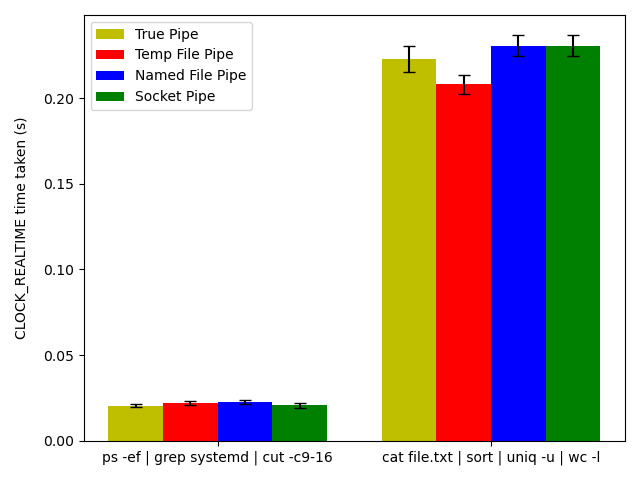
\includegraphics[width=0.95\linewidth]{12.png} \vspace{-0.1cm}
    \caption{\small Comparison of true pipes, temporary file pipes, permanent file pipes, and socket pipes on first pair of tested pipelines} 
    \label{fig12}
    \vspace{-0.3cm}
\end{figure}

\begin{figure}[!htp]
    \vspace{-0.0cm}
    \centering
    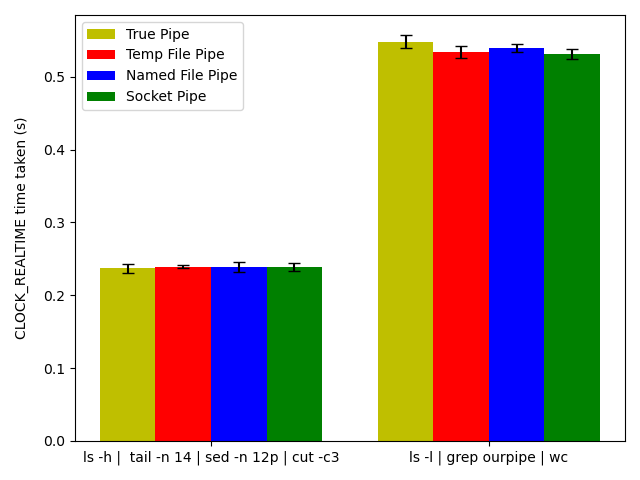
\includegraphics[width=0.95\linewidth]{34.png} \vspace{-0.1cm}
    \caption{\small Comparison of four pipe implementations on second pair of tested pipelines} 
    \label{fig34}
    \vspace{-0.3cm}
\end{figure}

\begin{table*}[!htp]
\centering
\begin{footnotesize}
\begin{tabular}{cccccc}
\toprule
    Pipeline & True Pipe & Temp File Pipe & Named File Pape &  Disk Sync & Socket Pipes \\ \midrule
    \texttt{ps -ef | grep systemd | cut -c9-16} & \makecell{0.0205 $\pm$ 0.0009s \\ 0 MB} & \makecell{0.022 $\pm$ 0.0012s \\ 0 MB} & \makecell{0.0228 $\pm$ 0.0012s \\ 0.06 MB} & \makecell{0.1523 $\pm$ 0.0017s \\ 0.06 MB} & \makecell{0.0206 $\pm$ 0.0016s \\ 0 MB}  \\
    
    \texttt{cat file.txt | sort | uniq -u | wc -l} & \makecell{0.223 $\pm$ 0.0076s \\ 0 MB} & \makecell{0.208 $\pm$ 0.0056s \\ 0 MB} & \makecell{0.2306 $\pm$ 0.0061s \\ 11 MB} & \makecell{19.0608 $\pm$ 7.2001s \\ 11 MB} & \makecell{0.2306 $\pm$ 0.0061s \\ 0 MB}  \\
    
    \texttt{ls -h |  tail -n 14 | sed -n 12p | cut -c3} & \makecell{0.2369 $\pm$ 0.006s \\ 0 MB} & \makecell{0.2391 $\pm$ 0.002s \\ 0 MB} & \makecell{0.2392 $\pm$ 0.0069s \\ 1.8 MB} & \makecell{4.4588 $\pm$ 0.4071s \\ 1.8 MB} & \makecell{0.2393 $\pm$ 0.0053s \\ 0 MB}  \\
    
    \texttt{ls -l | grep ourpipe | wc} & \makecell{0.5484 $\pm$ 0.0089s \\ 0 MB} & \makecell{0.5342 $\pm$ 0.0084s \\ 0 MB} & \makecell{0.5394 $\pm$ 0.0053s \\ 7.2 MB} & \makecell{19.3828 $\pm$ 6.543s \\ 7.2 MB} & \makecell{0.5313 $\pm$ 0.0069s \\ 0 MB} \\
    \bottomrule
\end{tabular}
\end{footnotesize}
\caption{\small Results of performing four pipelines on our file pipes and true Linux pipes} 
\vspace{-0.3cm}
\label{table1}
\end{table*}

\section{Discussion and Future Directions}

Overall, our project has been successful in terms of creating a working implementation of sequential piping using actual files, as well as an interactive shell program that a user can use to specify (almost) arbitrary pipelines. Furthermore, our socket pipes allow our pipelines to execute in parallel just like true Linux pipelines. Finally, we have gathered empirical data about the performance of different methods of IPC. If we were to return to this project in the future, we would attempt to replicate the parallel execution of true Unix pipes with our file pipes as well, implementing the desired blocking behavior and concurrency which is certainly much more difficult than implementing linear file pipes. This may require us to completely change our fork/exec framework; as stated we no longer have any direct control over the execution of a child process after it calls \texttt{execvp()}. Another shortcoming we have been unable to address is the usage of the single-quote character ' . There are programs that make significant use of this character, such as \texttt{awk}, that our program cannot handle. When the single-quote character appears in the arguments for any part of a specified pipeline, when the corresponding process eventually runs it (not our wrapper shell program) will throw an error saying that the single quote is an invalid character. Although we have been treating single quotes exactly the same as any other character, we probably need to change our approach in order to handle it.

In terms of evaluating our three file pipe implementations, we found that for all four of the pipelines we tested, our temporary file pipes gave very similar time performance to true pipes. Thus for pipelines consisting of simple filters, we conclude that sequential and parallel pipeline execution do not have any significant differences in overheads. In fact, sequential execution may be the reason why we saw more consistent performance in some of the pipelines, most notably \texttt{ls -h |  tail -n 14 | sed -n 12p | cut -c3}.  Furthermore, since a temporary file is immediately deleted after the last open file descriptor corresponding to it is closed, this approach incurs no permanent memory costs as expected. But if we store all pipe contents in permanent, named files, we would be able to analyze the outputs of earlier processes in a pipeline after execution has completed, among other possibilities. We did find that named file pipes introduced slight time overhead for all four tested pipelines, as expected. But the additional time taken was very slight to almost negligible in all cases. Thus we would not be dissuaded from using named files in place of temporary ones for time performance reasons, for pipelines consisting of simple filters. Perhaps more significant was the additional memory required to store all of the pipes in a pipeline. This was found to be fairly variable across our pipelines, being as high as $11$ MB for \texttt{cat file.txt | sort | uniq -u | wc -l} which is still a fairly simple pipeline. Thus temporary file pipes are preferred if running out of disk space is a concern. 

Also, Linux buffers all writes to disk which greatly improves performance when working with files, but this does decrease system reliability in case of crashes. We can improve reliability by forcing all writes to our permanent file pipes to be immediately synced to the disk. However, it is clear from all four pipelines that doing so incurs a very large performance overhead (especially when the files were relatively large as expected), and so this does not seem to be a good idea. Furthermore, we found that in several pipelines, forcing disk syncs resulted in highly inconsistent time performance, with some trials taking double to triple the usual amount of time. On the other hand, we found that socket pipes provided very similar performance for all four pipelines to true and temporary file pipes, and so we conclude that sockets do not introduce any inherent time overheads. Since our socket pipes also do not require any additional permanent storage and allow programs within a pipeline to be executed in parallel, we can say that socket pipes are actually the closest to the true underlying implementation of pipes and thus are preferred when we do not care to store pipe contents for future use.

Our endeavor of implementing and experimenting with file and socket "pipe" creation and in-shell usage in a programming language has been enlightening in several ways. Firstly, our choice to use C, motivated by its low-level capabilities and closeness to Unix systems, proved to be apt. It allowed us to delve into the intricacies of Unix pipes and their integration with the file I/O system. We thought about using a higher-level language to explore the implications of such a language choice; for example, both Python and Java provide POSIX system calls. This would likely simplify certain aspects but could obscure the essential systems details that C laid bare (e.g. parsing of command-line arguments), so we are happy with our choice of C. Our project also highlighted the importance of iterative development and testing in achieving functional goals. We initially implemented file pipes using a hard-coded pipeline of only two programs. After we were satisfied that our implementation worked, we extended this program to handle pipelines of arbitrary length.  We then created our custom shell wrapper program, which was capable of running user-supplied pipelines as well as allowing users to choose between our various pipe implementations. This provided a pragmatic and flexible approach to testing and comparison. Afterwards we were able to implement pipes using sockets and add this choice of implementation to our shell program. Overall, our work emphasized the importance of designing adaptable and modular software, especially in a research context where goals and requirements can rapidly evolve. 
\bibliographystyle{plain}
\bibliography{mybib}

\end{document}
